\section{Original frozen results}
\label{sec:results}
\subsection{No demonstrated primary benefit, with limited predictive signal}
Table~\ref{tab:primary} and Figure~\ref{fig:primary} give the frozen component comparison. The extension's paid-validation ridge area is slightly higher in both directions: $+0.5651\%$ K562 to RPE1 and $+0.0138\%$ RPE1 to K562. Both conditional query-resampling ranges cross zero. These observations show no demonstrated advantage in this replay; they neither establish equivalence nor rule out benefits under other splits, representations or budgets.

\begin{table}[htbp]
\centering\small
\caption{Frozen primary comparison. $A_E$ and $A_W$ are normalized MSE areas for the extension and worst-query, in units of $10^{-3}$. Difference $\Delta=A_E-A_W$ and its central 95\% conditional query-resampling range use units of $10^{-5}$. Positive values favor worst-query. Five acquisition-order/tie seeds share one fixed cell bank.}
\label{tab:primary}
\begin{tabular}{lrrrrr}
\toprule
Direction & $A_E$ & $A_W$ & $\Delta$ & Query range & Change (\%) \\
\midrule
K562$\to$RPE1 & 7.86844 & 7.82422 & +4.4212 & [-4.4957, +13.0315] & +0.5651 \\
RPE1$\to$K562 & 5.72383 & 5.72305 & +0.0789 & [-0.4150, +0.5948] & +0.0138 \\
\bottomrule
\end{tabular}

\end{table}

\begin{figure}[htbp]
\centering
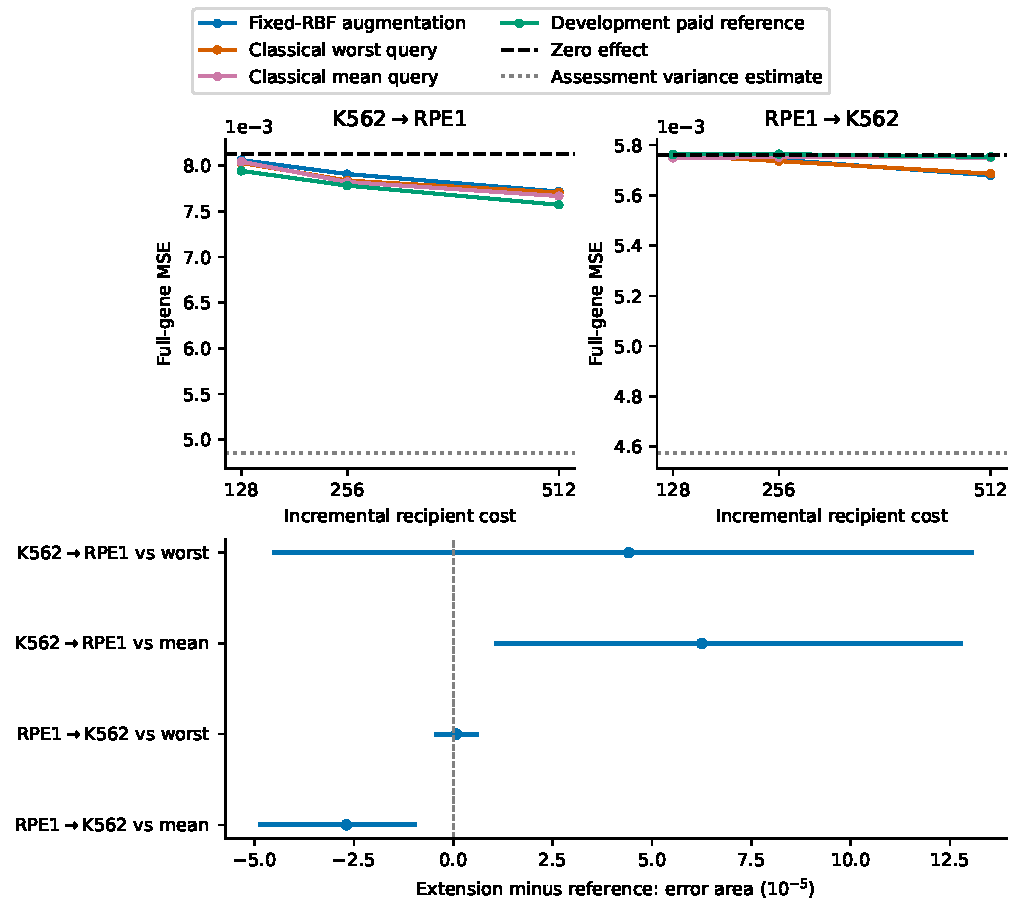
\includegraphics[width=\linewidth]{figures/primary-results.pdf}
\caption{Original real-data replay. Upper panels show observed MSE against abstract incremental recipient budget. Zero is a standalone zero-recipient-cost reference; its horizontal placement does not charge it the displayed purchases. The estimated assessment noise floor is plug-in context, not a known lower bound under arbitrary dependence. Lower panels show paired error-area differences and conditional query-resampling ranges, with all acquisition seeds averaged within query. Mean-query and worst-query use the same paid-validation ridge predictor. Development-selected reliability is a post-primary reference. Directions reuse observations; the ranges are not biological confidence intervals.}
\label{fig:primary}
\end{figure}

Comparator choice matters. Against mean-query, the extension changes area by $+0.8015\%$ forward and $-0.4678\%$ reverse, with conditional query ranges wholly above and below zero, respectively. Table~\ref{tab:devrefs} adds the development-selected references. The extension is $1.694\%$ worse than reliability/CV ridge forward and $0.623\%$ better reverse, with the latter range crossing zero. These post-primary comparisons cannot retrospectively replace the frozen hypothesis.

\begin{table}[htbp]
\centering\small
\caption{Post-primary comparisons with development-selected references. Differences and query ranges have units $10^{-5}$; negative changes favor the extension. Development's strongest overall point estimate was zero; reliability/CV ridge was its strongest paid combination. These are not new confirmatory tests.}
\label{tab:devrefs}
\begin{tabular}{llrrr}
\toprule
Direction & Development reference & Change (\%) & $\Delta$ & Query range \\
\midrule
K562$\to$RPE1 & Zero & -3.159 & -25.665 & [-47.096, -7.991] \\
K562$\to$RPE1 & Reliability/CV ridge & +1.694 & +13.106 & [+3.691, +23.889] \\
RPE1$\to$K562 & Zero & -0.623 & -3.590 & [-7.096, -0.774] \\
RPE1$\to$K562 & Reliability/CV ridge & -0.623 & -3.587 & [-8.563, +0.231] \\
\bottomrule
\end{tabular}

\end{table}

Observed zero-predictor areas are $.00812508$ and $.00575973$. The corresponding estimated scorer noise areas are $.00484897$ and $.00457337$, about $59.68\%$ and $79.40\%$ of zero error. Extension/ridge improves observed error over zero by only $3.159\%$ and $.623\%$. At budget 512 its gene-wise rank scores are $.07931$ and $.03856$, and raw direction cosines are $.08719$ and $.02784$. These weak scores and high measurement noise constrain biological interpretation. Noise subtraction is descriptive and does not turn a conditional resampling range into a population inference.

\subsection{Support, heterogeneity and source diagnostics}
An independent source-only audit finds rank five for all ten direction/seed pilot designs (four coordinates plus intercept), with all 131 query vectors in their estimated span. All 160 original policy trajectories share the same pilot prefix within direction/seed. Thus the original primary study tests precision allocation and shrinkage after estimated support, rather than recovery of an initially missing direction. The first 88 units are already spent before the budget-128 endpoint.

The paired-query distributions are heterogeneous (Figure~\ref{fig:influence}). Forward, 106/131 query-averaged differences favor worst-query and 25 favor the extension. Deleting any one query leaves the mean difference positive, ranging from $2.60\times10^{-5}$ to $7.13\times10^{-5}$. Reverse, 59 queries favor worst-query and 72 favor the extension; one leave-one-query-out deletion reverses the tiny positive aggregate. Individual acquisition-seed mean differences range from $-4.34\times10^{-5}$ to $1.82\times10^{-4}$ forward and $-2.20\times10^{-5}$ to $3.65\times10^{-5}$ reverse. These are dependence-aware descriptions, not independent seed replications. No query was excluded or used to choose a threshold.

\begin{figure}[htbp]
\centering
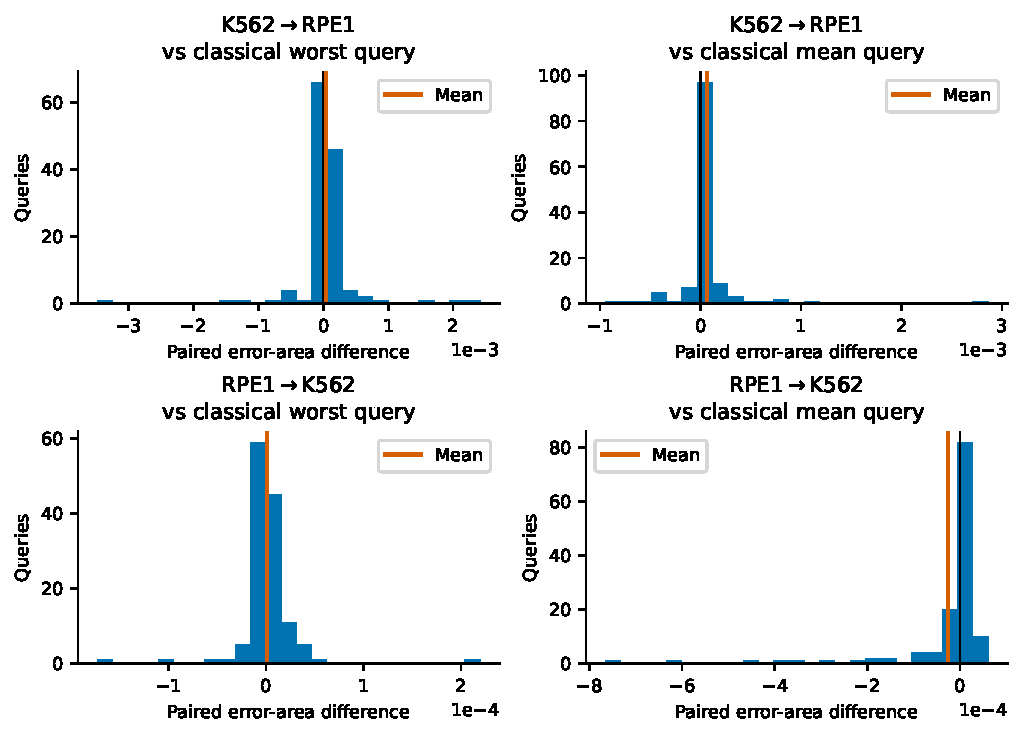
\includegraphics[width=\linewidth]{figures/query-contributions.pdf}
\caption{All 131 original paired query contributions per direction/reference, after averaging the five acquisition seeds. Negative values favor the extension. Orange lines mark means; they can differ from the median or majority sign. Histograms expose heterogeneity without changing the prespecified all-query endpoint. Queries share source estimation and assessment controls.}
\label{fig:influence}
\end{figure}

Source-warning heuristics flag 113/131 forward and 88/131 reverse queries. Retaining only unflagged queries would retain just 18 and 43, respectively, and can select harder queries rather than guarantee lower error. The original strong/weak-source strata and all retention denominators remain available; weak source response does not prove a null recipient effect. Source-identity permutation moves extension/ridge areas to $.00812767/.00576257$; query-source gene permutation gives $.00805871/.00576258$. These controls weaken intervention-specific transfer, but global offsets and shrinkage can survive corruption. Source-half sensitivity and support checks are diagnostics, not calibrated certificates.

Ordinal and absolute accuracy also differ. The reconstructed transport comparator has worse absolute-error area than the local network under all 16 policies in each direction, yet some centered specificity/rank metrics improve. Source copy has reverse rank score $.06820$, exceeding paid ridge's $.03856$ despite much worse absolute error. Table~\ref{tab:ranking} reports common denominators. These observations do not reproduce or refute PerturbMap's published result under its different implementation and task.

\subsection{Known-truth failures and conditional successes}
Across the 14 original controlled scenarios, the extension's true-error area is higher than worst-query in ten and lower in four. The baseline change is $+1.41\%$, while the nonlinear-shift case improves by $5.08\%$; all world-level uncertainties and scenarios are retained in Table~\ref{tab:all-scenarios}. Five generated worlds supply the independent Monte Carlo units, and scenarios reuse those worlds. In all 25 matched baseline/nonlinear world/acquisition-seed pairs, allocation sequences are identical. Hence the nonlinear improvement is conditional alignment of a fixed geometry-based allocation with a changed error surface, not detection of nonlinear bias. All 350 zero-weight/worst-query ledger pairs are byte-identical, verifying the component ablation.

Figure~\ref{fig:failures} illustrates a support counterexample. With an exact missing source direction, all 150 query/seed records are correctly unsupported; after source-coordinate error, all 150 appear estimated-supported while none is oracle-supported. This is a constructed failure, not an estimate of its prevalence in real screens. The same distinction affects uncertainty: for fixed ridge/worst-query at budget 192, nominal 95\% coverage is $.954$ in the baseline, $.864$ under nonlinear shift and $.781$ under source-feature error of standard deviation one. Widths fail to track the added structural error. These idealized Gaussian diagnostics are not a proposed valid adaptive inference method.

\begin{figure}[htbp]
\centering
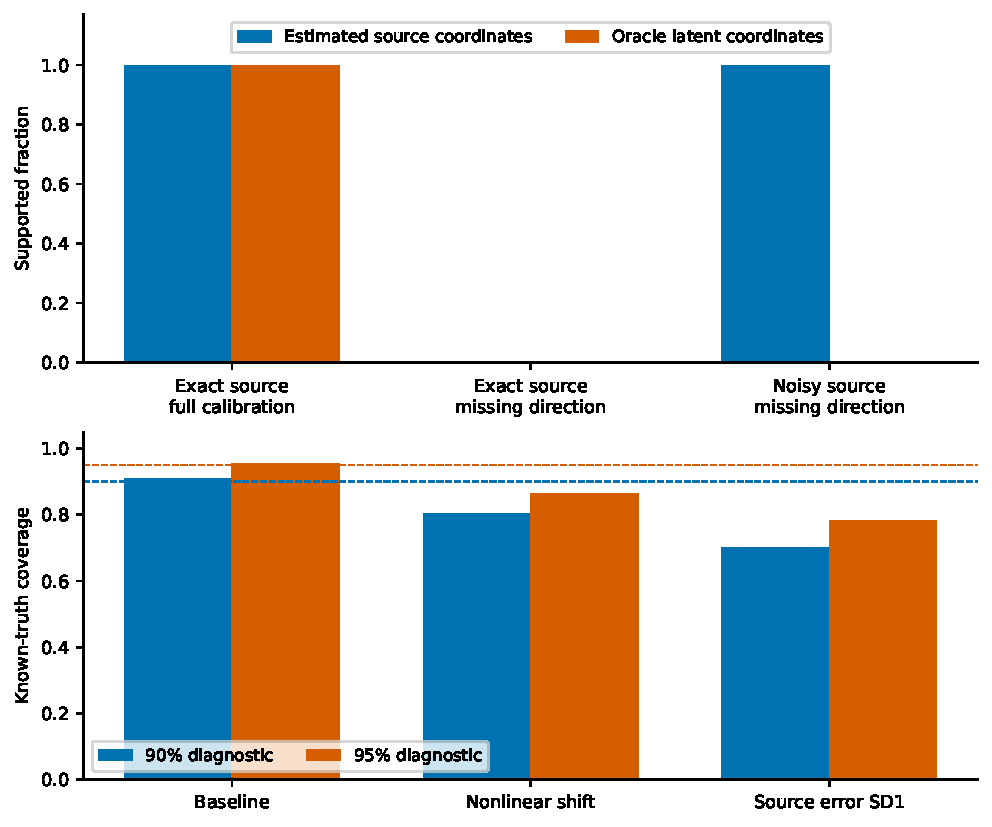
\includegraphics[width=\linewidth]{figures/support-and-coverage.pdf}
\caption{Known-truth support and coverage diagnostics. Upper panel: estimated versus oracle support for six queries across five acquisition seeds and five worlds at the final budget; 150 records are dependent observations, not independent worlds. Source-coordinate error can conceal a missing direction. Lower panel: empirical coordinate coverage of nominal 90/95\% intervals centered on fixed-ridge predictions, conditional on finite width. Baseline, nonlinear-shift and source-error settings separate sampling variance from omitted structural error. Complete widths and undefined counts appear in Table~\ref{tab:intervals}.}
\label{fig:failures}
\end{figure}

Price sensitivity and direct query measurement are supplementary (Appendix~\ref{app:assessment}). They do not establish real monetary savings or a universal budget boundary.
